\section{Motivation}
%\begin{itemize}
%    \item Machine Hearing Principles
%    \item Spectrogram Based Machine Hearing
%    \item Case for Audio-Based Machine Hearing (w/ results teaser)
%\end{itemize}

We begin with an overview of machine hearing principles and make the case for 
an audio-centric CBAR technique.

\subsection{Machine Hearing Principles}

Machine hearing is an emerging field focused on endowing machines with  
the ability to hear as humans do~\cite{lyon-human-2017}.
%However, this field has lagged behind computer vision due to its seeming lack
% of general applicability. 
%This is shown by the wealth of specialized music and
%speech sound analyses, with more general problems being ignored. 
The goal is to formulate a generalized model of sound with associated
representation, classification, and retrieval techniques. 
The architecture of an audio DBMS for machine hearning, that is inspired by the
human auditory system, consists of three components~\cite{lyon-machine-2010}:

\PP{Representation}
The first component, peripheral analyzer, is based on a part of the inner ear,
called \textit{cochlea} \footnote{Outer-ear structures are at the mercy of the
recording medium (\eg, the microphone).}. 
This spiral-shaped cavity is responsible for forming a representation of the 
given audio data.
by transforming acoustics into neural signals.
\textit{Reissner's membrane} is an important cochlear structure that can be
considered as a collection of band-pass filters, separating sounds into spectral
components~\cite{Plack2018}. These spectral components are then processed by
brain structures that convert the waveform representation to a more compact one.
 
The next step consists of creating an image representation of the given audio
data, thereby modeling the concept of human auditory sensory memory (\ie, echoic
memory) \AJ{Cite}.
The perception of sound depends on what comes before and occurs after an audio
segment. Thus, echoic memory determines human perception. 
It is critical in permitting the listener to integrate incoming information
with past events\footnote{Researchers have not reached consensus on the duration
of the memory  with estimates ranging from 250~ms to four
seconds~\cite{Wingfield2016}.}.
It is challenging to achieve high retrieval accuracy with only the image
representation and as such the next component is used for extracting key
features.

\PP{Classification}
The second component consists of feature extraction module that construct a more
compact and meaningful representation from the image formed by the previous
component.
This module most closely matches the \textit{neural code} of human audio
perception which forms the interface between sound and its conscious perception.
We note that the human auditory processing pipeline is still mostly unknown
and much of what we do know is speculative. 
It is hypothesized that multiple processes occur in
sequence to prepare the information for perception \cite{Eggermont2001}. 
It is likely these processing steps make actual perception less computationally
expensive. The output of this component determines the performance and
efficiency of the final component.

\PP{Retrieval}
This component takes in the representation formed by the previous module 
and maps it decisions. This component is analogous to conscious perception in
humans. It can vary from simple (\eg, a single perceptron) to complex
structures (\eg, a deep neural network).

\subsection{Image-Based Machine Hearing}
% \begin{itemize}
%     \item How this fits into Neural Coding and Echoic Memory
%     \item CNN approach
%     \item Autoencoding CNN approaches
%     \item Image retrieval (PAMIR approach)
% \end{itemize}

Given the high accuracy of content-based image retrieval (CBIR) systems, 
researchers have attempted to leverage these systems for audio retrieval.
This technique consists of transforming audio recordings to spectrograms and
subsequently use image retrieval techniques for audio retrieval.
Thus, it leverages machine vision to perform machine hearing, thereby 
combining the neural coding and echoic memory portions of human hearing 
into a single step \footnote{The vision model is directly trained on
spectrograms instead of relying on a separate classification module.}.

\begin{figure}[!tbp]
    \centering
    \subfloat[Noisy]{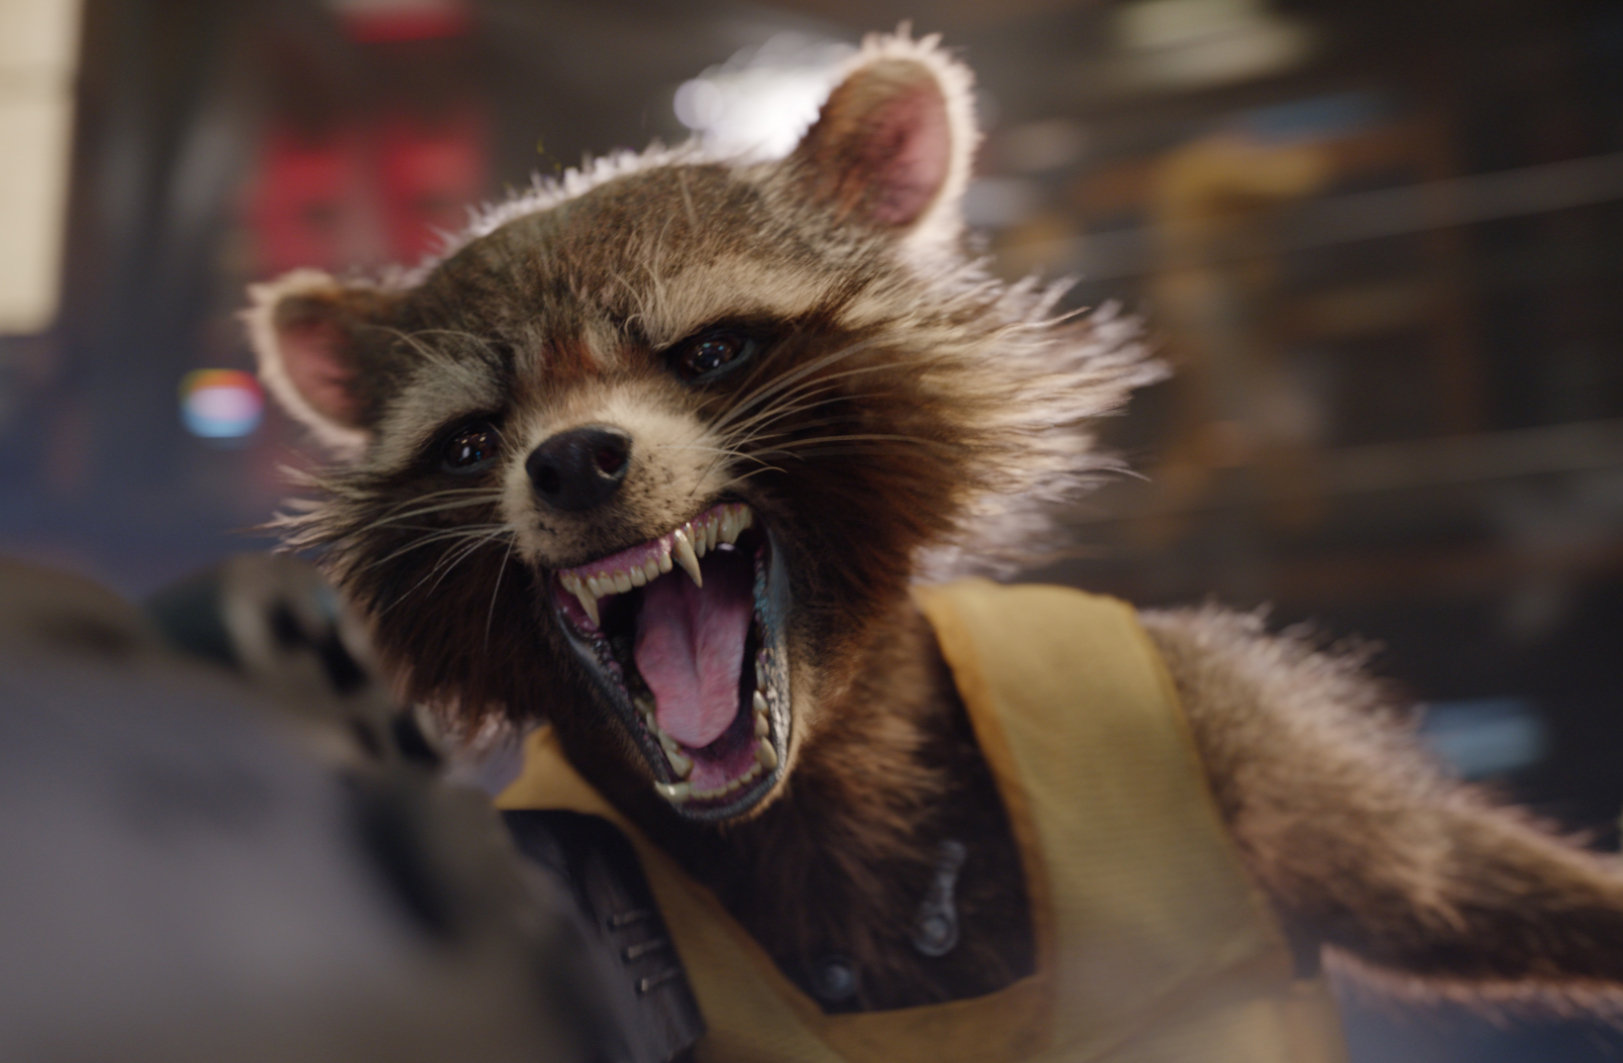
\includegraphics[width=0.4\textwidth]{figures/noisy-audio.jpg}\label{fig:noisy-audio}}
    \hfill
    \subfloat[Clean]{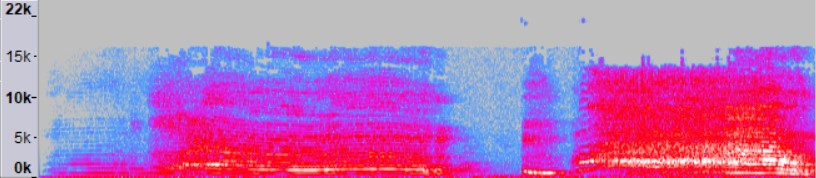
\includegraphics[width=0.4\textwidth]{figures/clean-audio.jpg}\label{fig:clean-audio}}
    \caption{Spectrograms illustrating the difference between clean and noisy audio when converted to visual domain.}
    \label{fig:noisy-audio-cmpr}
\end{figure}

This approach for translating audio to a visual domain has seen some success,
especially in cases where audio events are isolated as illustrated
in~\cref{fig:noisy-audio-cmpr}.
However, in real-world audio recordings are typically generated from multiple
audio sources often with overlapping frequencies (\eg, group meetings).
This challenge stems from the \textit{transparency} of audio unlike images. 
Thus, a spectrogram is analogous to placing several transparent images 
over one another. 
State-of-the-art CBAR systems use a convolutional neural network (CNN) for 
image classification\AJ{Cite, describe CNN in a few sentences} and
train the CNN model on spectrograms.
However, these systems are unable to deliver high accuracy (> 70\%) even with
complex model ensembles~\cite{xu-large-scale-2018,piczak-environmental-2015}.

A more recent development in image-based machine hearing is to use an
unsupervised learning technique called auto-encoding. An auto-encoder is a
neural network that is half of a reconstruction network in which an image is
reduced to latent variables and reconstituted. Often, the spectrogram is reduced
to latent variables using CNNs. Again, while CNNs have success in image
recognition, the same issues arise as discussed before. Additionally, relevant
data is likely ignored and thus can cause even worse performance especially in
mixed source documents.

In an attempt to capitalize on image retrieval success, Chechik et al. used
spectrogram imagery to perform unstructured audio retrieval with
passive-aggressive model for image retrieval (PAMIR) \cite{Chechik2008}. This
work used probabilistic confidence to rank audio documents on relevance to a
text query. When tested against the Freesound database though it saw no
improvement over GMM or SVM using traditional audio features. The average
precision of the classifier was 0.27 with a max of about 0.55.

\subsection{Waveform-Based Machine Hearing}
% \begin{itemize}
%     \item Naive audio features
%     \item DTW + HMM
%     \item Autoencoding RNN approaches
%     \item Biologically Based Encoding
%     \item My approach + some teaser
% \end{itemize}
Perhaps the most common audio representation used in classification tasks is the
Mel-frequency cepstral coefficients (MFCCs). They are popular because they are
cheap to calculate and provide a representation that is consistent with human
hearing \cite{kaur-feature-2015}. Many specific tasks are successful using only
MFCCs however for a general case of audio representation, more information is
needed. For this, a naive approach is to extract the temporal and spectral
features from the waveform to provide a more complete representation. Though,
this approach is costly and leads to greater data dimensionality causing
classification agents to converge more slowly.

Other approaches like Dynamic Time Warping (DTW) and Hidden Markov Models (HMMs)
work directly on the audio data-stream itself and thus do not require feature
extraction or spectral image creation. These approaches have found success in
both speech recognition and specialized retrieval systems. Both DTW and HMMs
have the benefit of taking into account the sequential nature of the audio data
when making a determination. However, DTW is a costly algorithm and in the
context of large databases is infeasible for use. Similarly, HMMs can become very
complex especially when needing to determine many classes as a model needs to be
trained for each class. Additionally, neither take advantage of domain knowledge
and do not conform to the machine hearing principles outlined above.

While auto-encoding with CNNs saw little success, Recurrent neural network (RNN)
based encoders preform well. This is due to much of the information in audio
being reliant on what comes before it. Unlike CNN based encoders, RNN based
encoders do not encode the spectrogram image but instead can learn from the
waveform values or vectors of spectrogram features presented as a time series.
This kind of auto-encoder has the benefit of being cheap to compute and creating
compact representations that take time into account and can be used with any
number of off-the-shelf classifiers.

The biological neural code for audio encoding has been sought even before
machine hearing was solidified as a field \cite{Eggermont2001}. Through studies
of the biological systems that convert sound waves to neural responses,
researchers have been able to emulate some portions with others requiring
speculation. Smith and Lewicki give a nonlinear model based on population spike
code to encode waveforms \cite{smith-efficient-2006}. In this work, they
illustrate that idealized spikes encode precise temporal positions and
magnitudes of underlying acoustic features. This work provides a method to
extract an efficient coding of natural sounds, making sure the classifiers are
working with the most information dense representation possible.

\begin{table}[t]
    \centering
    \begin{tabular}{ccc}
         & 250   & 2000  \\ \hline
    DNN  & 0.174 & 0.191 \\
    HDNN & 0.246 & 0.130
    \end{tabular}
    \caption{Simple table with audio representations and their complexity/usefulness/features}
    \label{tab:audioreps}
\end{table}